\documentclass[a4paper,10pt]{article}


\usepackage[bottom]{footmisc}

%\documentclass[a4paper,12pt,pdflatex]{article}
\usepackage[table]{xcolor}
\usepackage{longtable} % Thsi sort of tables can break accrooss pages repeating the header
\newcolumntype{L}[1]{>{\raggedright\let\newline\\\arraybackslash\hspace{0pt}}m{#1}}
\newcolumntype{C}[1]{>{\centering\let\newline\\\arraybackslash\hspace{0pt}}m{#1}}

\usepackage{makecell}	
\usepackage{helvet}
\renewcommand{\familydefault}{\sfdefault}
\usepackage[compact, pageatnewline]{titlesec}
\setlength{\baselineskip}{2\baselineskip}
\usepackage{lipsum}			% ability to insert dummy text
\usepackage{multicol}
\usepackage[utf8]{inputenc}
\usepackage{enumitem}
\usepackage{xcolor}
\usepackage{parallel}
\usepackage{siunitx}
\usepackage{booktabs}
\usepackage{fancyhdr}
\usepackage{stackengine}			% needed to stak thing in header
\usepackage{vmargin}
\setstackEOL{\\}
\usepackage{libertine}
\usepackage{array,arydshln}
\usepackage[section]{placeins}
\usepackage[export]{adjustbox}
\usepackage[T1]{fontenc}
\usepackage{underscore}
\usepackage[euler]{textgreek}
\usepackage{lastpage} % to get lastpage
%\usepackage{tabularx} % allows defining the table width (whole page for instance)
\usepackage{ltablex}%\usepackage{tabulary}
\usepackage{gensymb}
\usepackage{csvsimple} % allows reading csv files
%\usepackage{pgfplotstable} 
\usepackage{colortbl} % This allows to color the first line of tables
\usepackage{xhfill}
\newcounter{magicrownumbers} % This is a counter for rownumbers 
\newcommand\rownumber{\stepcounter{magicrownumbers}\arabic{magicrownumbers}}
\setlength\parindent{0pt}

\usepackage{framed}
\newcommand\VRule[1][\arrayrulewidth]{\vrule width #1}
\renewcommand*\familydefault{\sfdefault}  %% Only if the base font of the document is to be sans serif
\renewcommand*{\hrulefill}[2][0pt]{\leavevmode \leaders \hbox to 1pt{\rule[#1]{1pt}{#2}} \hfill \kern 0pt} % Macro to redefine table lines 

\usepackage[]{hyperref}
\newcolumntype{Y}{>{\centering\arraybackslash}X}

\newenvironment{Figure}
  {\par\medskip\noindent\minipage{\linewidth}}
  {\endminipage\par\medskip}
  
\usepackage{multirow} % 15/06/2020 for datasheet
\usepackage{pbox}
\usepackage{subfig}
%\usepackage{subcaption}
%\usepackage{caption}
 
 \setlist[itemize]{leftmargin=* ,noitemsep, topsep=0pt} % configures itemize to remove vertical spaces 
%\usepackage{subcaption}
%\usepackage{subfloat}
\usepackage{titlesec}
%\usepackage[flushleft]{threeparttable}
\titlespacing*{\section}{0pt}{0.2\baselineskip}{0.2\baselineskip}
\titlespacing*{\subsection}{0pt}{0.5\baselineskip}{0.2\baselineskip}


%%%%%%%%%%%%%%%%%%%%%%%%%%%%%%%%%%%%%%%%%%%%%%%%%%%%%
%%% DOCUMENT Information, %%%
%%%%%%%%%%%%%%%%%%%%%%%%%%%%%%%%%%%%%%%%%%%%%%%%%%%%

%\newcommand{\theproject}{NEUROPV}
\newcommand{\doctype}{ REFERENCE DESIGN }
\newcommand{\docinfo}{   }
\newcommand{\chipID}{XZL}

%\newcommand{\blockID}{OTA-CHOPPED-00}
\newcommand{\DOCref}{APN-000029}

% initial Versionning info
\newcommand{\thedate}{March-2021}
\newcommand{\CopyrightYear}{2021}
\newcommand{\DOCiss}{rev. 1.0}
\newcommand{\theauthor}{G.Laurent}
\newcommand{\Change}{New document}
\newcommand{\blockID}{} 

\title
{ \begin{framed}
		\hspace{100 mm} \\
		\theproject - \chipID \\
		\thetitle \\
		\hspace{100 mm}
	\end{framed}
}

\date{}
%\author{\theauthor }

\setmarginsrb{2cm}{1cm}{2cm}{1cm}{60pt}{0.5cm}{30pt}{1cm} % SET DOCUMENT MARGINS: \setmarginsrb{leftmargin}{topmargin}{rightmargin}{bottommargin}    {headheight}{headsep}{footheight}{footskip}


%%% First page  HEADER %%%
%--------------------------------------------------------------------------------
\fancypagestyle{firststyle}
{
\lhead{\begin{tabular}[b]{l}  \raisebox{-.5\height}{\raggedleft 
\includegraphics[width=3cm]{inputs/LOGOHorizontal.png}} \\  { \footnotesize  \textbf{\href{https://www.vddtech.com} {\color{black} {www.vddtech.com}}}}  \end{tabular}} %  {\footnotesize \textbf{control your power }}
\rhead{\begin{tabular}[b]{r}    \\ {\normalsize \textbf{ \chipID}} \\ {\small  \DOCref {} - \DOCiss {} - \thedate}  \end{tabular}}
\chead{\begin{tabular}[b]{c}   \\  \doctype \\ \docinfo {}   \end{tabular}}


\fancyfoot[l]{  \pbox{120pt} {\scriptsize{Copyright © \CopyrightYear, VDDTECH}}}
\fancyfoot[r]{   \thepage {} of \pageref{LastPage}} % \thepage\of \pageref{LastPage}
\fancyfoot[c]{\footnotesize{  \textbf{VDDTECH} }}

\renewcommand{\headrulewidth}{2pt}
\renewcommand{\footrulewidth}{2pt}
}

%%% DOCUMENT HEADER %%%
%--------------------------------------------------------------------------------
\lhead{\begin{tabular}[b]{l}  \raisebox{-.5\height}{\raggedleft 
\includegraphics[width=3cm]{inputs/LOGOHorizontal.png}} \\  { \footnotesize  \textbf{\href{https://www.vddtech.com} {\color{black} {www.vddtech.com}}}}   \end{tabular}} %  \\ {\footnotesize \textbf{control your power }}
\rhead{\begin{tabular}[b]{r}    \\ {\normalsize  \textbf{\chipID}} \\ {\small \DOCref {} - \DOCiss {} - \thedate}  \end{tabular}}
\chead{\begin{tabular}[b]{c}  \\  \doctype \\ \docinfo {}  \end{tabular}}

\fancyfoot[l]{    \pbox{120pt}{ \scriptsize{Copyright © \CopyrightYear, VDDTECH} } }
\fancyfoot[r]{   \thepage {} of \pageref{LastPage}} % of \pageref{LastPage}
\fancyfoot[c]{  \footnotesize{  \textbf{VDDTECH}  }}

\renewcommand{\headrulewidth}{2pt}
\renewcommand{\footrulewidth}{2pt}

\titleformat{\section}{\bfseries\Large\raggedright}{}{0em}{\MakeUppercase} % this allow making section title in CAPITALS 

\setlist[itemize]{leftmargin=* ,noitemsep, topsep=0pt} % set default options for itemize

%%%%%%%%%%%%%%%%%%%%%%%%%%%%%%%%%%%%%%%%%%%%%%%%%%%%%%%%%%%%%%%%%%%%%%%%%%%%%%%%%
%%% DOCUMENT TITLE %%%
%%%%%%%%%%%%%%%%%%%%%%%%%%%%%%%%%%%%%%%%%%%%%%%%%%%%%%%%%%%%%%%%%%%%%%%%%%%%%%%%%
%\documentclass{article}

%\documentclass[a4paper,12pt,pdflatex]{article}

\begin{document}

%\vspace*{150pt}
%{\let\newpage\relax\maketitle}
%\maketitle
\thispagestyle{firststyle}

\newpage
\pagestyle{fancy}



%\setlength{\baselineskip}{\baselineskip}
\section*{\centerline{  HHHHHHHHH }  }% 3000Vpk, 200kV/\textmu s removed
\vspace{-20pt}
\section*{\centerline{  with VDDTECH  components}  }
\vspace{-20pt}
\noindent\hrulefill{2pt}

%%%%%%%%%%%%%%%%%%%%%%%%%%%%%%%%%%%%%%%%%%%%%%%%%%%%%%%%%%%%%%%%%%%%%%%%%%%%%%%%%%
%%% Document information

\begin{multicols}{2}
%\twocolumn	
\section*{FEATURES}
	\textbf{
		{\normalsize    
			 %\begin{itemize}[leftmargin=* ,noitemsep, topsep=0pt] % Option to have items not separated
\begin{itemize}	
	\item IZL-100 digital Isolators \footnote{see ABS-000022 datasheet} % {\footnotesize (see ABS-000022)}
	\item NZL-300 transformer driver \footnote{see ABS-000023 datasheet} %{\footnotesize (see ABS-000023}) 
	\item  IZL-200 Isolated error amplifier \footnote{see ABS-000024 datasheet} %{\footnotesize (see ABS-000024)}
	\item HARSH environment 
	\item high switching frequency
	\item High Voltage 
		\end{itemize}}
	}

vdsnkvndkslvnskdnvklsnklnkdsvsd,vdskmv,nksdlnvlkdss q 


dsvkdspokvsodpvkodspv,sp


	\vfill\null
	
	\columnbreak
	%\vspace{-20pt}
\section*{DESCRIPTION}	
The Green Phase-Shifted Full-Bridge is a high efficiency ZVS resonant converter 


Maximizes power density 

optimizes power transformer

compact high switching frequency 

using state of the art GAN switches 

Low EMI 

through the use of decentralized floating voltages 



is reliable (no opto ) high temperature components 





%  \noindent
%\begin{minipage}{\columnwidth}
%	\makeatletter
%	\newcommand{\@captype}{figure}
%	\makeatother
%	\centering
%	\subfloat[Digital isolator pinout]{%
%		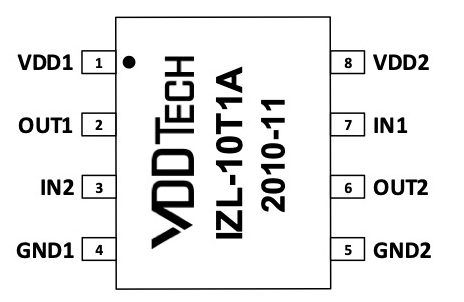
\includegraphics[width=0.45\columnwidth]{imgDS/IZL10T1AComp.png}%
%		\label{fig:evaluation:revenue}%
%	}\qquad%
%	\subfloat[Digital isolator symbol]{%
%		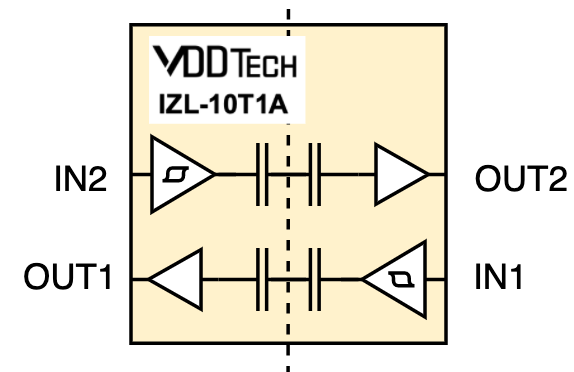
\includegraphics[width=0.45\columnwidth]{imgDS/IZL10T1ASymb2.png}%
%		\label{fig:evaluation:avgPrice}%
%	}
%%	\caption{Simulation results}
%\end{minipage}
%	\vfill\null
%	\noindent
	
%\begin{figure}[!htb]
%	\begin{minipage}{\columnwidth}
%	\centering
%	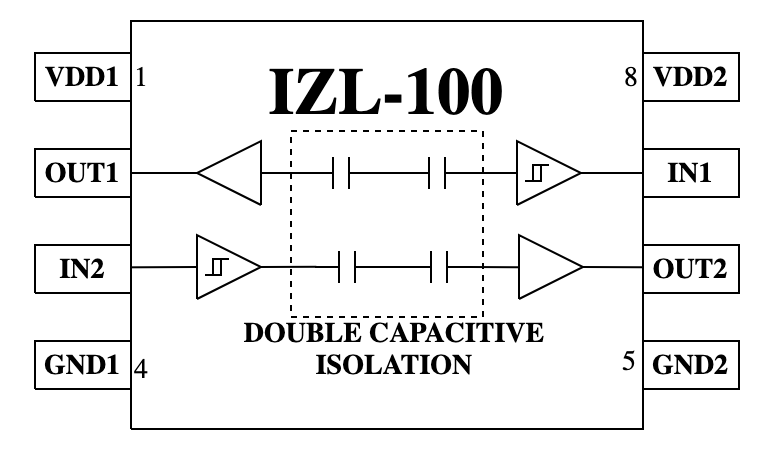
\includegraphics[max height=5cm,max width=0.95\columnwidth]{imgDS/IZL100.png}% requires the graphicx package
%
%	%\caption{simplified Schematic of 1 Channel. }
%%	\label{fig.:simplifiedschematic}
%%\captionsetup{width=.4\linewidth}
%%\caption{Simulation results}
%\end{minipage}
%\end{figure}

	%\vspace{-15pt}
\end{multicols}
%\end{twocolumn}

%\onecolumn

%\setlength{\parskip}{0.2em}
%\vspace{-1.5\baselineskip}
%\medskip
%\section*{DESCRIPTION}
%The \chipID {} Evaluation Board is an open loop Buck converter designed to demonstrate VDDTECH's \chipID {} digital isolator capability in terms of CMTI. This Buck converter features state of the art GAN 650V switches which are controlled through VDDTECH's digital isolators. 

\begin{figure}[!htb]
	\centering
	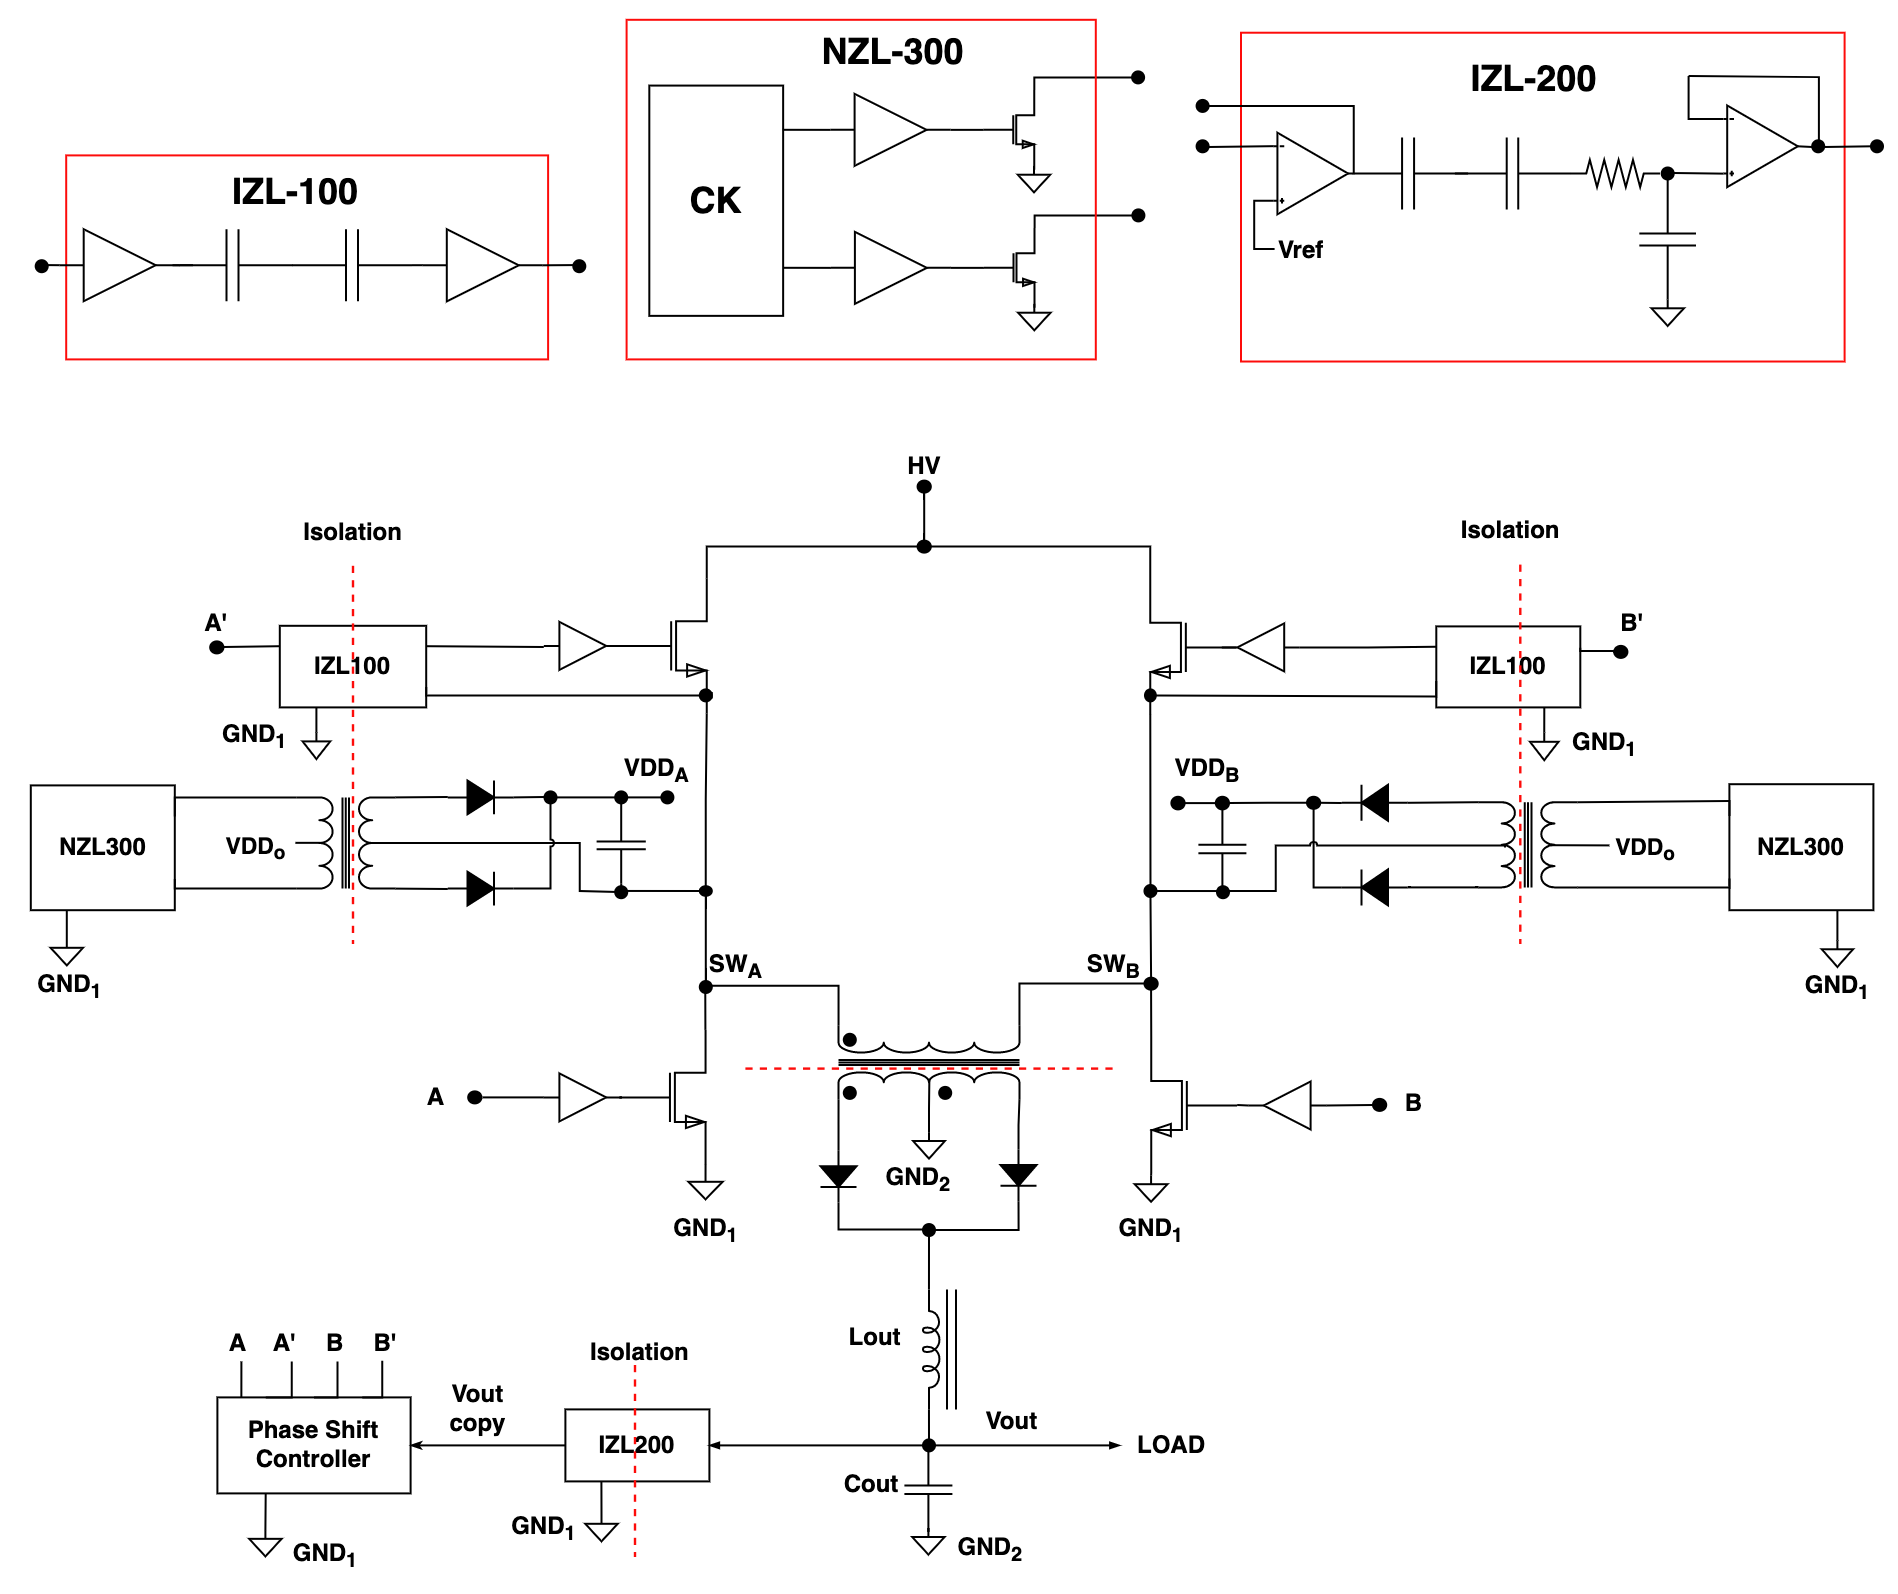
\includegraphics[max height=14cm,max width=17cm]{imgDS/Application3.png} 
%	\caption{\chipID {} Functional schematic illustration. }
	\label{fig BlockDiagram2}
\end{figure}

%\vfill\null

%\pagebreak

%\begin{figure}[!htb]
%	\begin{minipage}[t]{0.5\linewidth}
%		\centering
%		\captionsetup{width=0.9\linewidth}
%		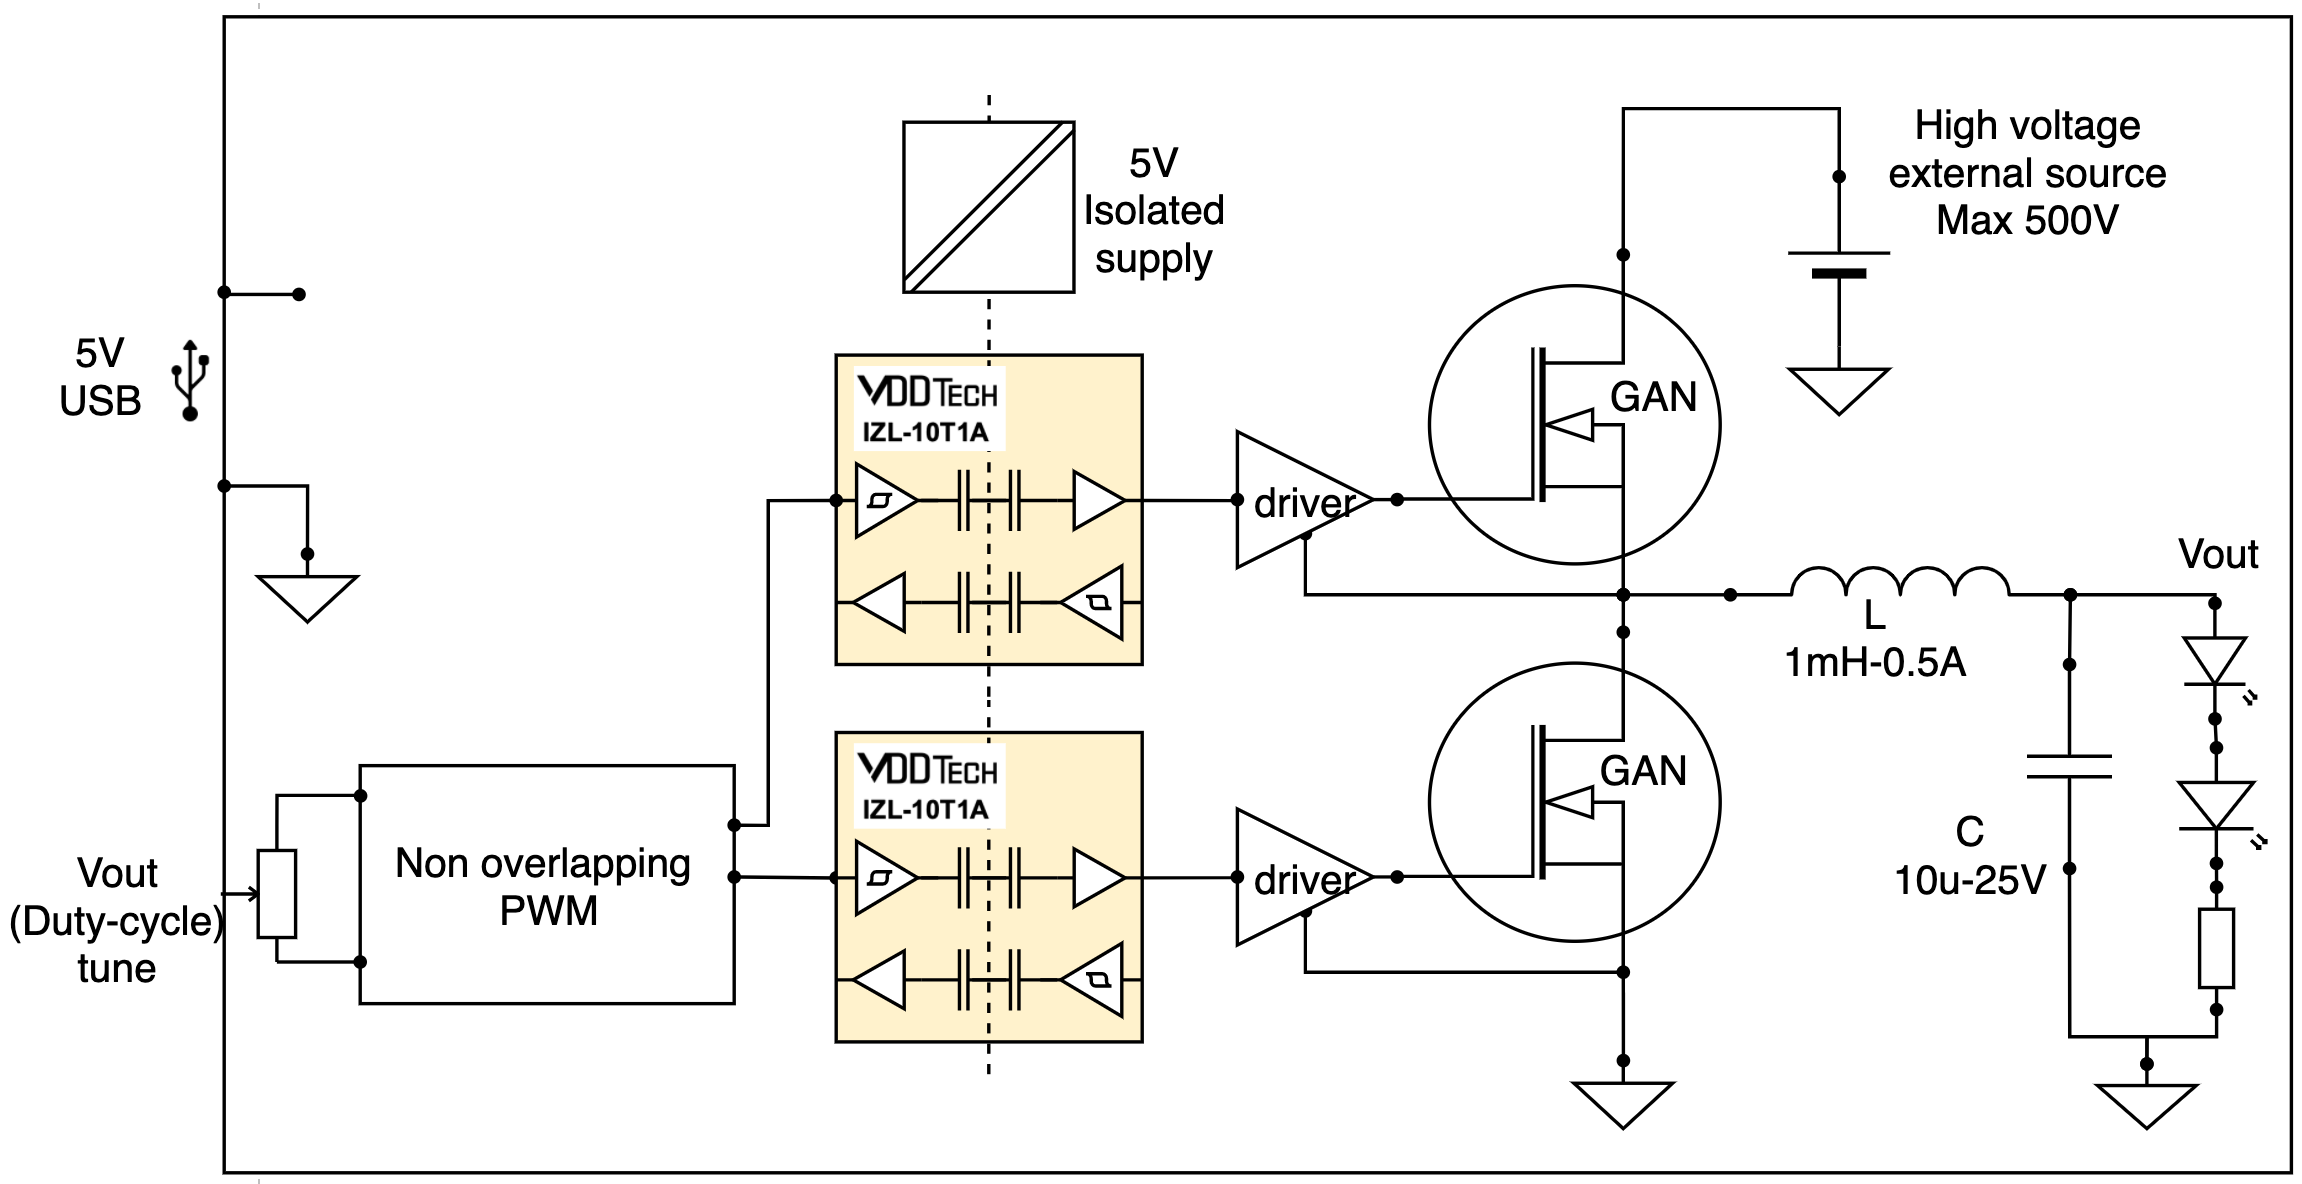
\includegraphics[max height=5cm,max width=0.95\linewidth]{imgDS/BlockDiagram2.png}% requires the graphicx package
%		\caption{ \chipID {} Functional schematic illustration. }
%		\label{fig.:SupplyVSDR}
%	\end{minipage}
%	\begin{minipage}[t]{0.5\linewidth}
%		\centering
%		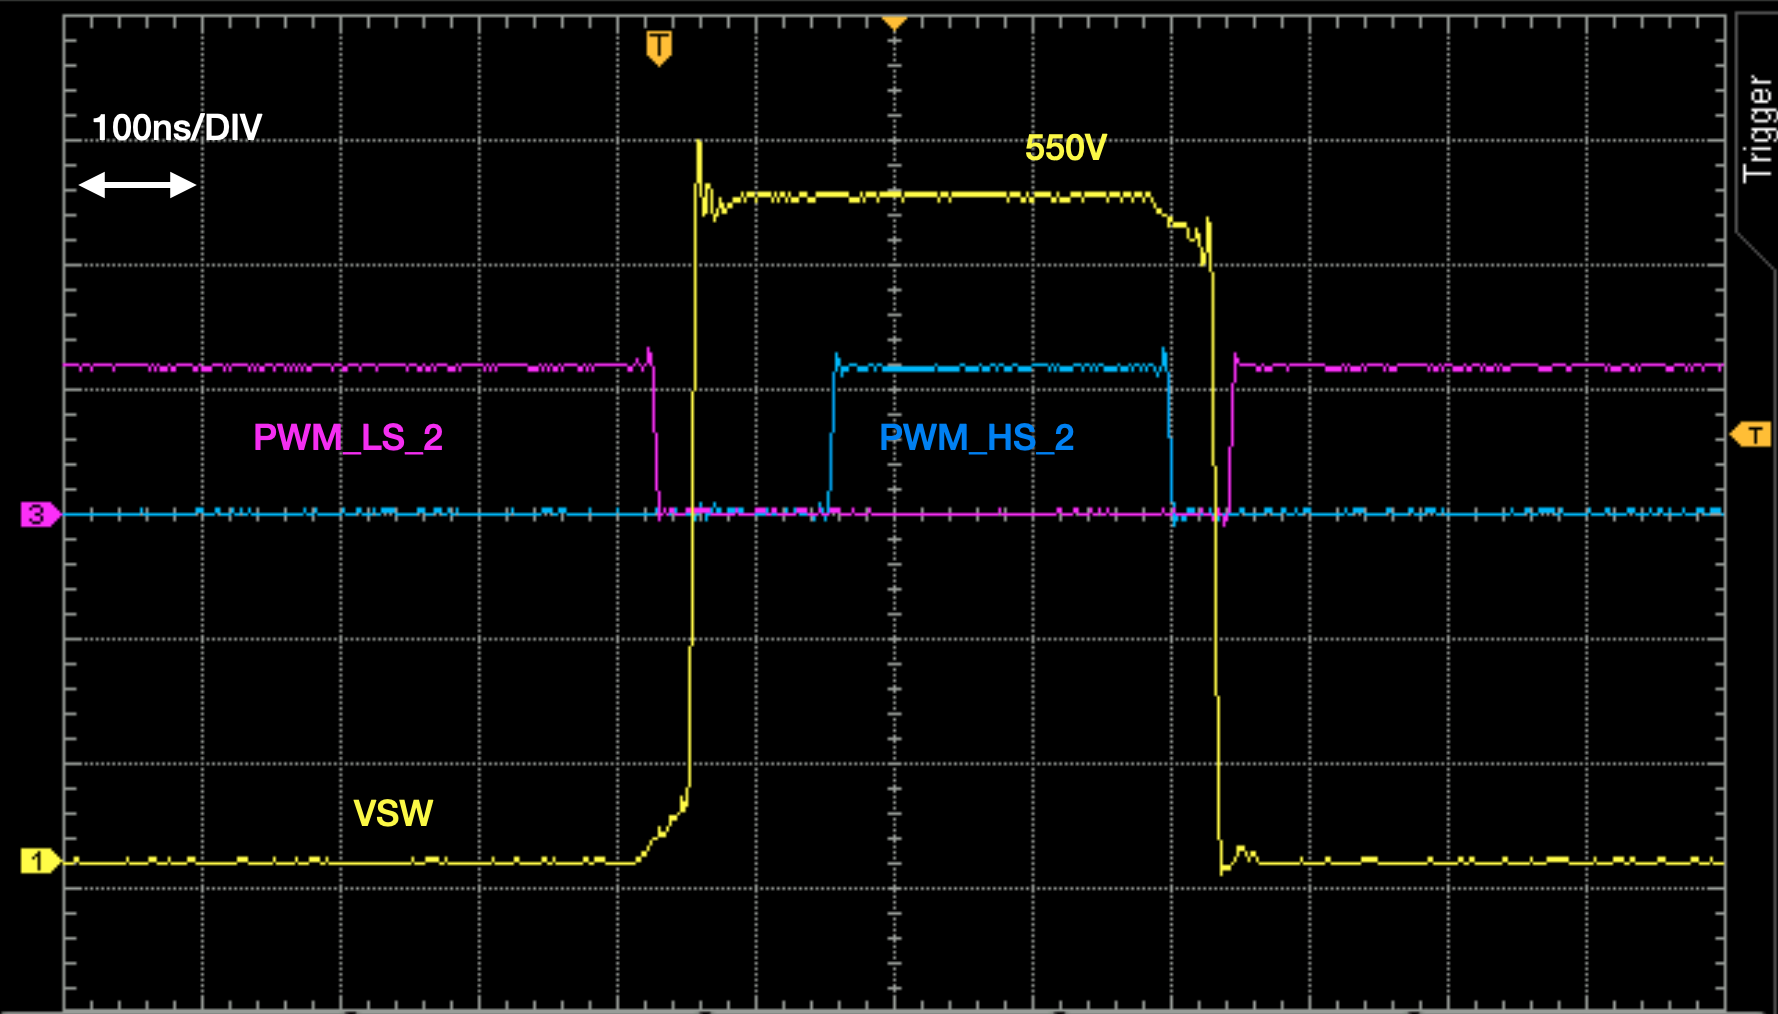
\includegraphics[max height=5cm,max width=0.95\linewidth]{imgDS/DemoExample.png}% requires the graphicx package
%		\captionsetup{width=.9\linewidth}
%		\caption{Switching node illustration (yellow): DVDT = 100KV/ \textmu s}
%		\label{fig.:functional}
%	\end{minipage}
%\end{figure}

\pagebreak
\newpage


%\section{VDDTECH's \chipID {}  overview}
%Figures \ref{fig IZL10T1AComp} and \ref{fig IZL10T1ASymb2} provide an illustration of respectively the pinout and the symbol view of the \chipID. 
%
%The \chipID {}  is a dual-channel digital isolator. This device has 1 forward and 1 reverse channel. The isolator is based on the integrated VDDTECH’s double capacitive isolation barrier, providing galvanic isolation up to 3000 Vpk and sustaining more than 200kV/μs transient immunity. The internal proprietary modulation technique combined with the small isolation capacitance (200fF per channel) provide fast operation (up to 40Mb/s), reduce EMI and self-correct the output state within 250ns in case of corrupted data, always ensuring the proper DC level of the output. 
%
%The \chipID {} features a protection which prevents the output to accidentally toggle if a fast DVDT event (faster than 1KV/\textmu sec) occurs. It means that if the input data toggle while a fast DVDT is occurring, the corresponding output won't toggle immediately.  %The output will be updated either within the 250ns refresh rate or if other input data transients occur without new DVDT event. 

%\begin{figure}[!htb]
%	\begin{minipage}[t]{0.5\linewidth}
%		\centering
%		\captionsetup{width=0.9\linewidth}
%		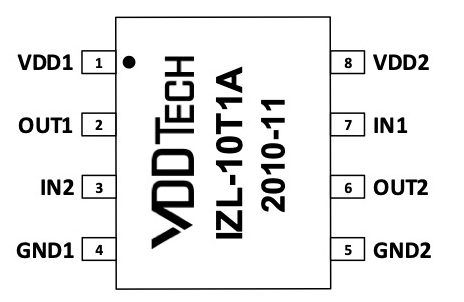
\includegraphics[max height=5cm,max width=0.95\linewidth]{imgDS/IZL10T1AComp.png}% requires the graphicx package
%		\caption{ \chipID {} -  pinout illustration. }
%		\label{fig IZL10T1AComp}
%	\end{minipage}
%	\begin{minipage}[t]{0.5\linewidth}
%		\centering
%		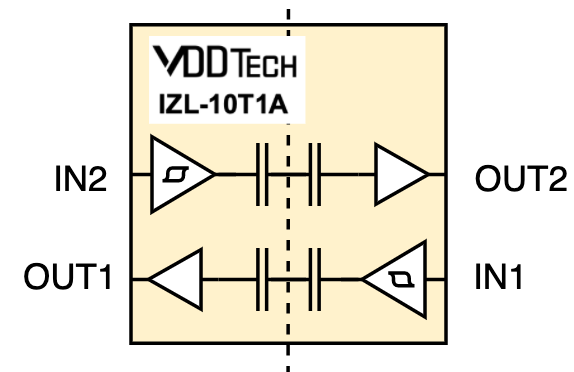
\includegraphics[max height=5cm,max width=0.95\linewidth]{imgDS/IZL10T1ASymb2.png}% requires the graphicx package
%		\captionsetup{width=.9\linewidth}
%		\caption{\chipID {} -  symbol representation.}
%		\label{fig IZL10T1ASymb2}
%	\end{minipage}
%\end{figure}


%\begin{figure}[!htb]
%	\centering
%	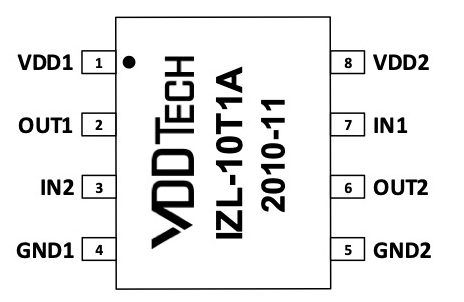
\includegraphics[max height=8cm,max width=14cm]{imgDS/IZL10T1AComp.png} 
%	\caption{\chipID {} -  pinout illustration. }
%	\label{fig.:IZL10T1AComp}
%\end{figure}
%
%\begin{figure}[!htb]
%	\centering
%	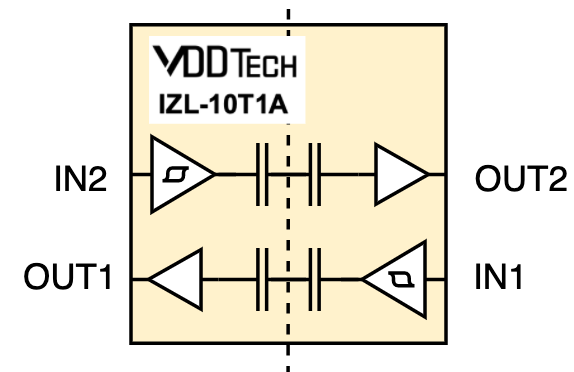
\includegraphics[max height=8cm,max width=14cm]{imgDS/IZL10T1ASymb2.png} 
%	\caption{\chipID {} -  symbol representation. }
%	\label{fig IZL10T1ASymb2}
%\end{figure}
%
%\FloatBarrier
%\clearpage
%\newpage
%\pagebreak

%
%\section{ZVS Evaluation Board }
%
%\begin{figure}[!htb]
%	\centering
%	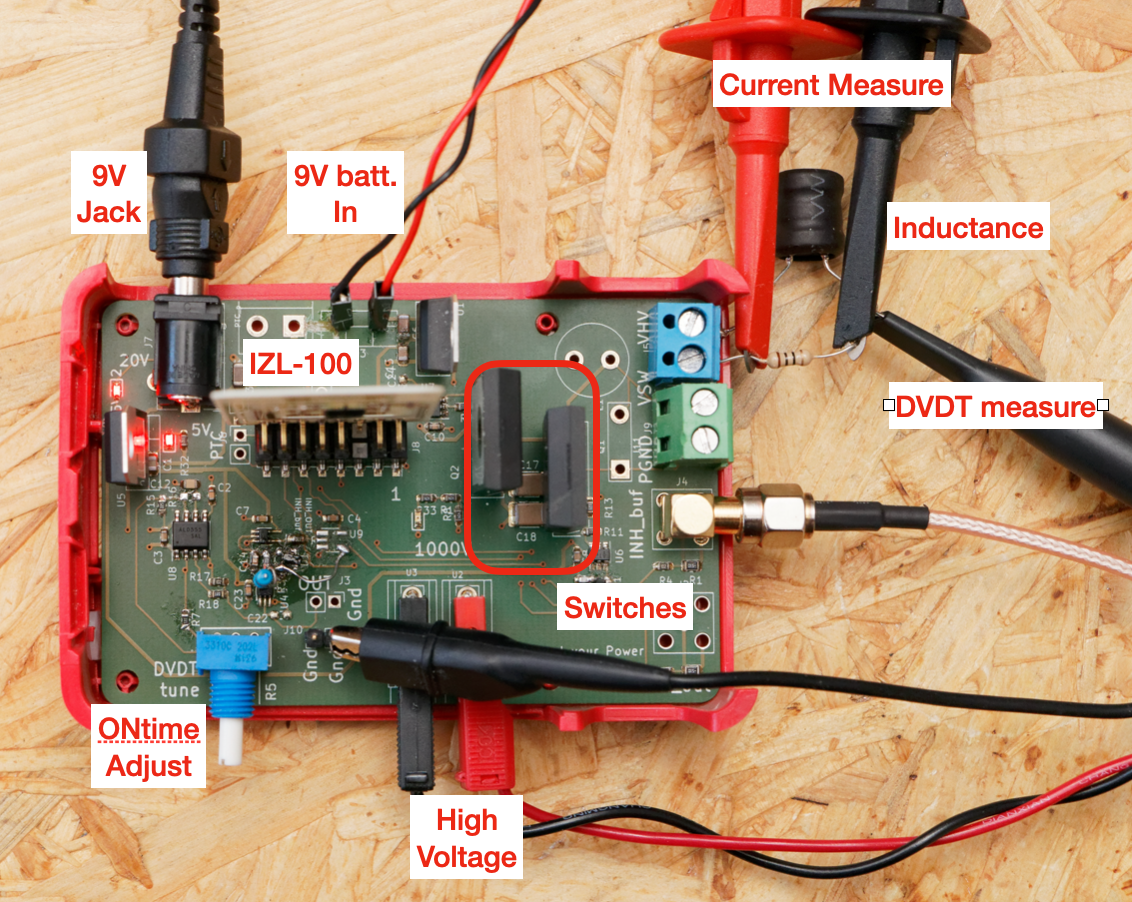
\includegraphics[max height=8cm,max width=14cm]{imgDS/setup2.png} 
%	\caption{\chipID {} -  ZVS evaluation board measurement interface. }
%	\label{fig.:symbol}
%\end{figure}
%
%\FloatBarrier

%\subsection{Interfaces table}
%{\small
%	\setcounter{magicrownumbers}{0} 
%	\renewcommand{\arraystretch}{1.4}
%	\begin{tabularx}{\linewidth}{|l|l|p{0.2\linewidth}|X|}
%		\caption{\chipID {} - Interfaces description.}\label{tab:IOdescription}  \\ 		\hline
%		\rowcolor{lightgray} {}  & Interface   & Connector & Description  \\ 		\hline
%		\endhead
%		\rownumber & USB 5V 		& female Micro-USB B-type & female Mirco-usb connector for 5V power supply input.     \\ \hline
%		\rownumber & High Voltage & 2mm female Banana Jacks & Input voltage range  [0-550VDC]. nominal Input current < 1mA. \newline \textbf{Current limit on voltage source should be inferior to 10mA}. \\ 	\hline
%		\rownumber & VOUT adjust & POTENTIOMETER (screw)  & Turning this potentiometer can slightly adjust the output voltage by tuning the PWM dutycycle.   \\ 		\hline
%		\rownumber & PWM_HS_2 & SMA RF connector  & Provides an image of the High side Gate Drive voltage. Signal Amplitude is 200mV.   \newline typical frequency=30KHz- 1\%Duty-Cycle  \\ 		\hline
%		\rownumber & PWM_LS_2  &  SMA RF connector  & Provides an image of the Low side Gate Drive voltage. Signal Amplitude is 200mV.   \newline typical frequency=30KHz- 98.5\%Duty-Cycle  \\ 		\hline
%		\rownumber & PWM jumper &  Pin Header  			& Leave Jumper in place to allow internal non-overlapped PWM signal. If open output voltage falls at 0V.     \\  		\hline
%		\rownumber & PWM EXT &  SMA RF connector  & WAS used during initial testing. Not connected.     \\ 		\hline
%		\rownumber & DVDT measure &  Vias (VSW, GND)   & Measuring access to switching node (VSW) for DV/DT measurement. Measurement is illustrated in Figure \ref{fig.:MeasurementIllustration2}    \\ 		\hline
%	\end{tabularx}
%}


%\FloatBarrier
%\clearpage
%\newpage
%\pagebreak

%
%\section{Observed signals and explanation }
%
%Measurable signals are illustrated in Figure \ref{fig.:Measurements}. Buck switching node is accessible on two vias located next the the Low-Side GAN. The two RF connectors provide an image (through the second channel of the digital isolators) of the PWM signals sent to the High and the Low side GAN. They are named respectively PWM_HS_2 and PWM_LS_2. Figure \ref{fig.:DVDTmeasurement} illustrates the measurement setup of the switching node VSW (for DV/DT extraction) and the measurement of the image (PWM_HS_2 and PWM_LS_2) of input signals of the High-side and Low-Side GAN drivers.   
%
%\begin{figure}[!htb]
%	\centering
%	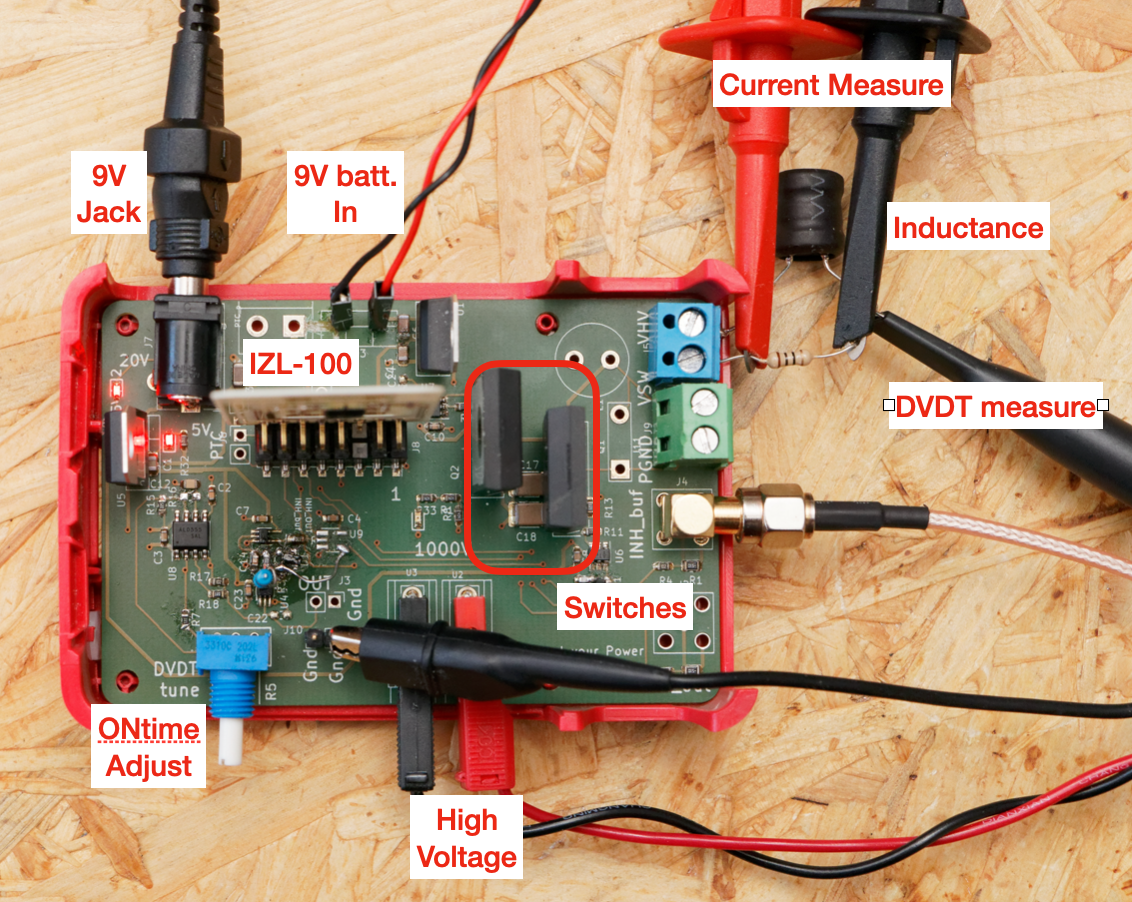
\includegraphics[max height=12cm,max width=17cm]{imgDS/setup2.png}
%	\caption{\chipID{ } -  Evaluation Board: Block view of the available measurements.}
%	\label{fig.:Measurements}
%\end{figure}
%
%\begin{figure}[!htb]
%	\centering
%	\includegraphics[max height=10cm,max width=17cm]{imgDS/DVDTMeasurement2.png}
%	\caption{\chipID{ } -  DVDT practical measurement setup illustration.}
%	\label{fig.:DVDTmeasurement}
%\end{figure}
%
%Before showing the measurement results, the time diagram of Figure \ref{fig.:FigSRC01BuckGAN} sketches the expected main internal signals. Looking for exemple on PWM_LS input signal, it generates the PWM_LS_1 signal with a typical 30ns delay relative to the forward path of the \chipID {}  digital isolator. Next, this PWM_LS_1 signal goes both to the LS driver (generating VGS_LS with a small driver delay) and to the reverse digital isolator channel to generate the PWM_LS_2 signal. It is this last signal that is measured on a SMA connector of the Eval Board.
%It is exactly the same logic for the PWM_HS input signal. However, the rising edge of the VGS_HS signal generates a fast rising transient on the Buck switching node VSW. If this fast transient occurs while PWM_HS_1 just toggled,  the digital isolator output PWM_HS_2 goes to memory state to avoid wrong toggling during fast DVDT event. %After the DVDT event, the digital isolator will regenerate automatically its correct state within a 250ns delay. 
%This is represented by the unknown state on PWM_HS_2 signal on the time diagram. The most important is that internal PWM_LS_1 and PWM_HS_1 signals are corrects. 
%
%\begin{figure}[!htb]
%	\centering
%	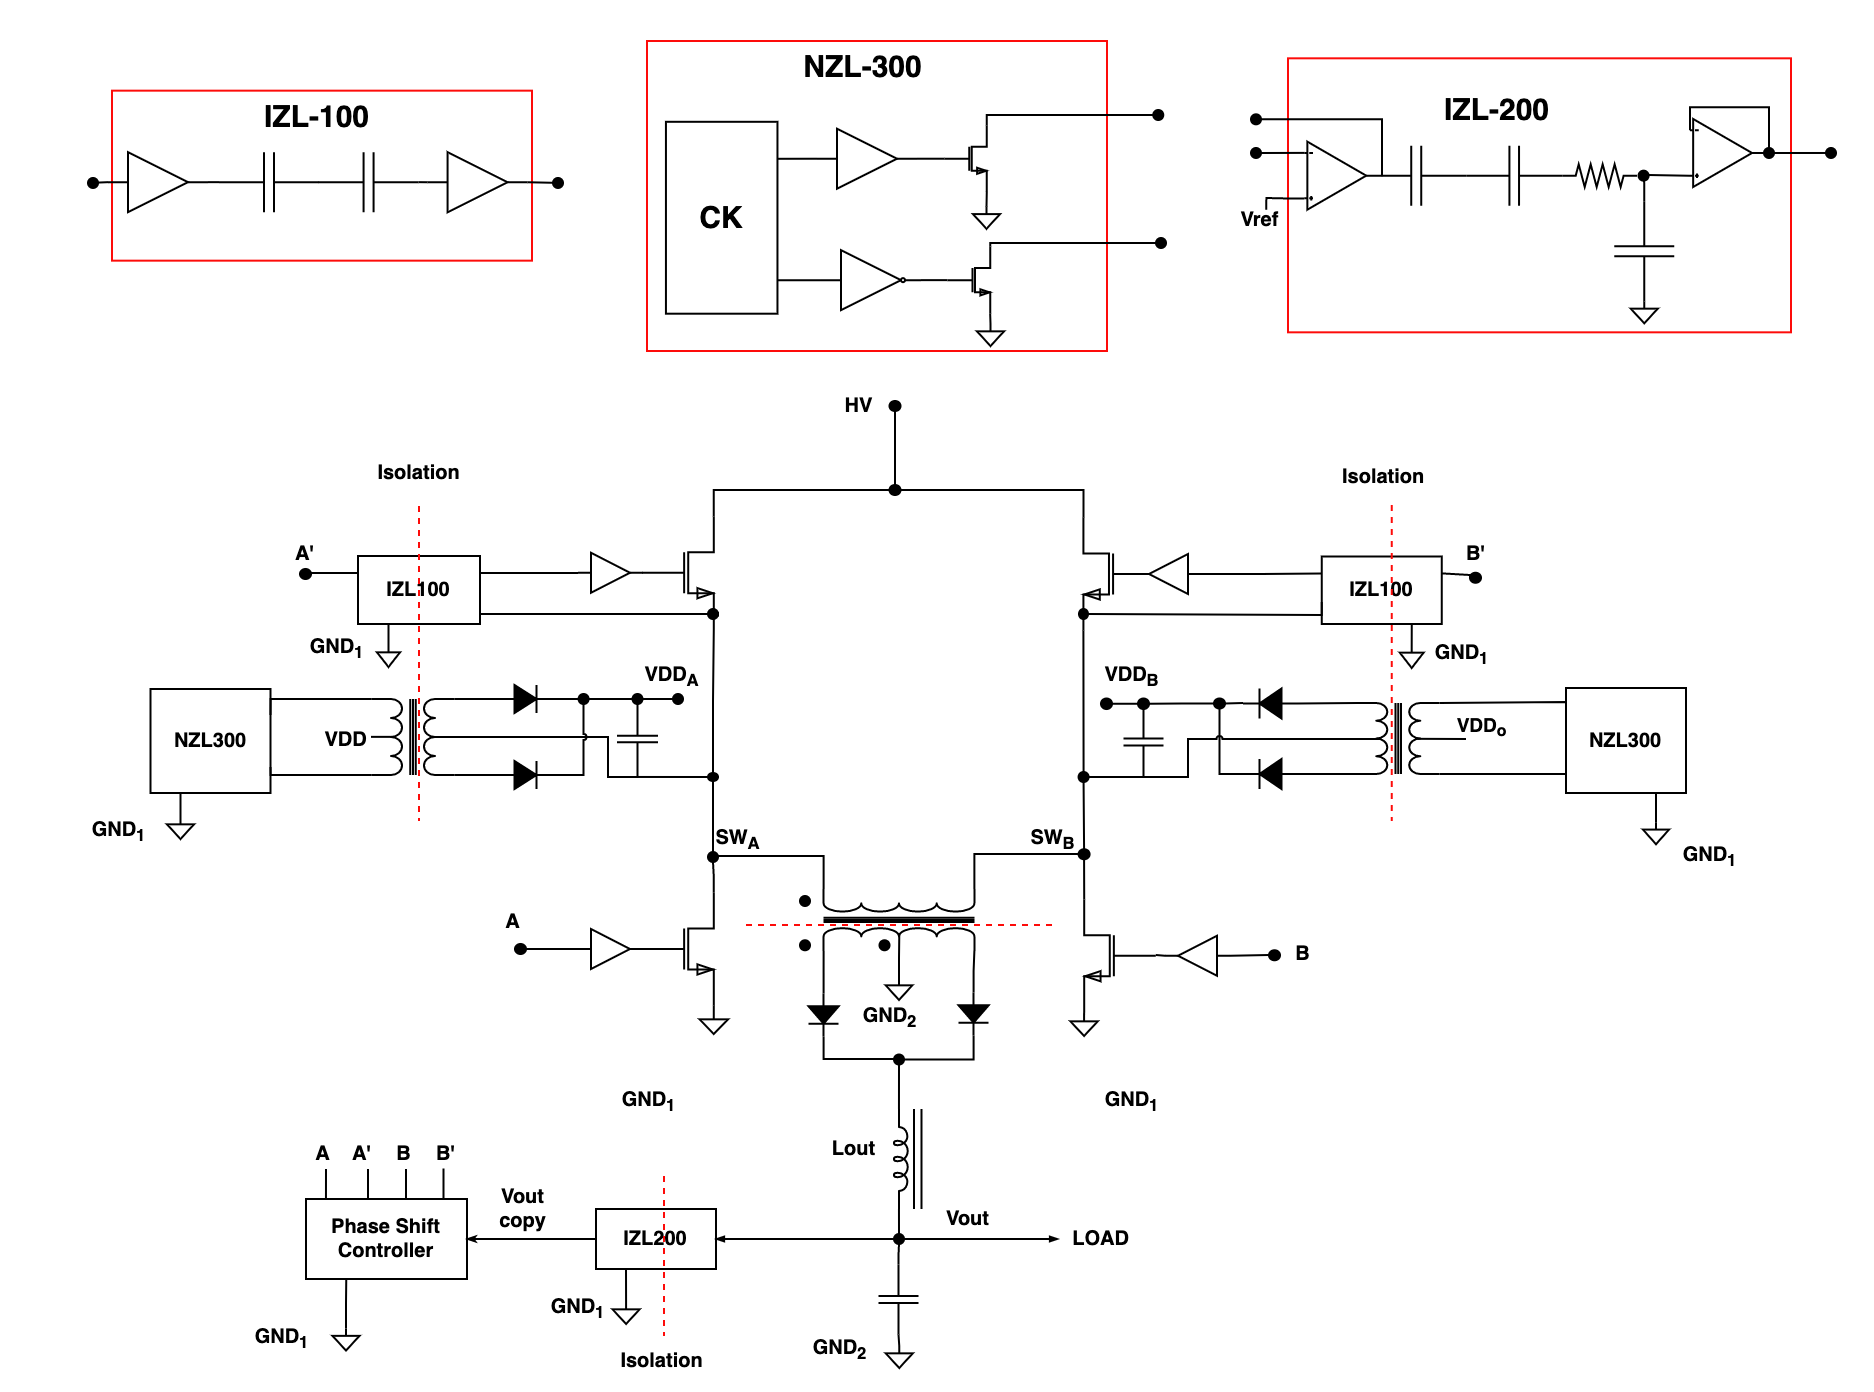
\includegraphics[max height=12cm,max width=17cm]{imgDS/Application2.png}
%	\caption{\chipID{ } -  Evaluation Board: expected main internal signals.}
%	\label{fig.:FigSRC01BuckGAN}
%\end{figure}
%
%
%Figure \ref{fig.:MeasurementIllustration2} is a measurement corresponding to PWM_LS_2 (magenta), PWM_HS_2 (blue) and VSW (yellow). Measured waveforms are compliant with our previous time diagram. There is also no visible jitter in these measured signals as expected.   
%

%\begin{figure}[!htb]
%	\centering
%	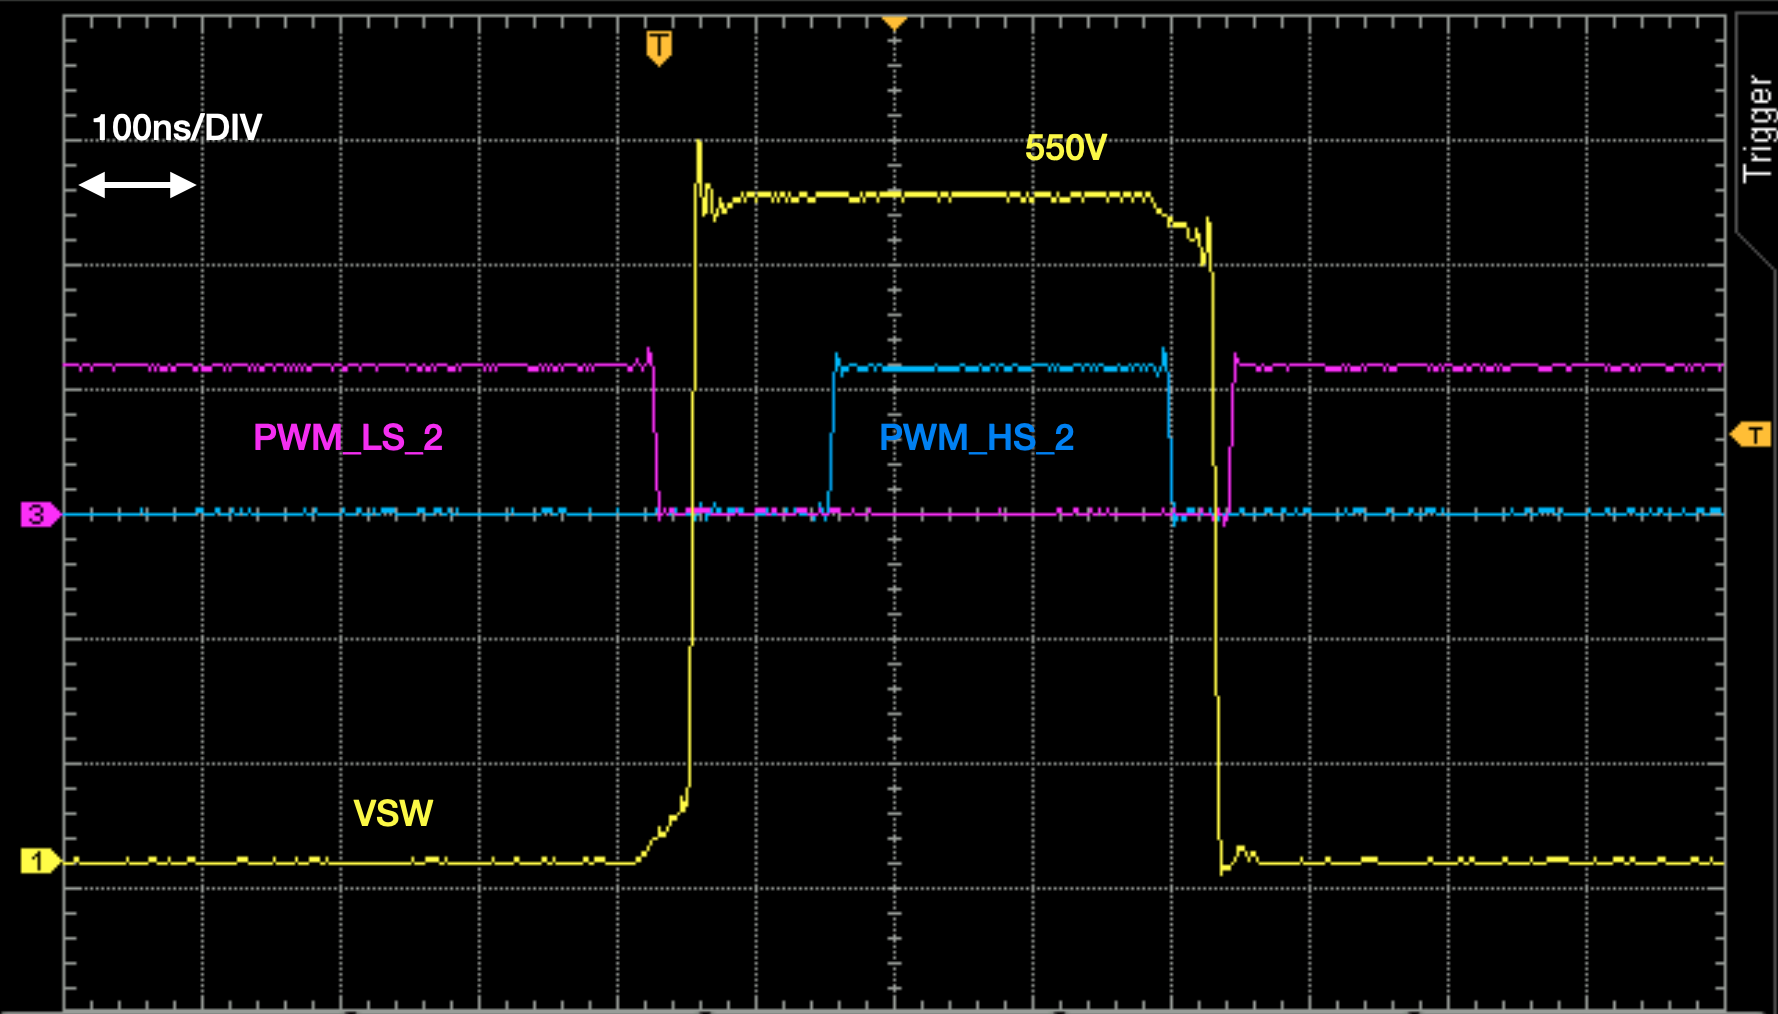
\includegraphics[max height=14cm,max width=17cm]{imgDS/DemoExample.png}%MeasurementIllustration3.png}
%	\caption{\chipID{ } -  DVDT measurement illustration.}
%	\label{fig.:MeasurementIllustration2}
%\end{figure}

%\begin{figure}[!htb]
%	\begin{minipage}[t]{0.5\linewidth}
%		\centering
%		\captionsetup{width=0.9\linewidth}
%		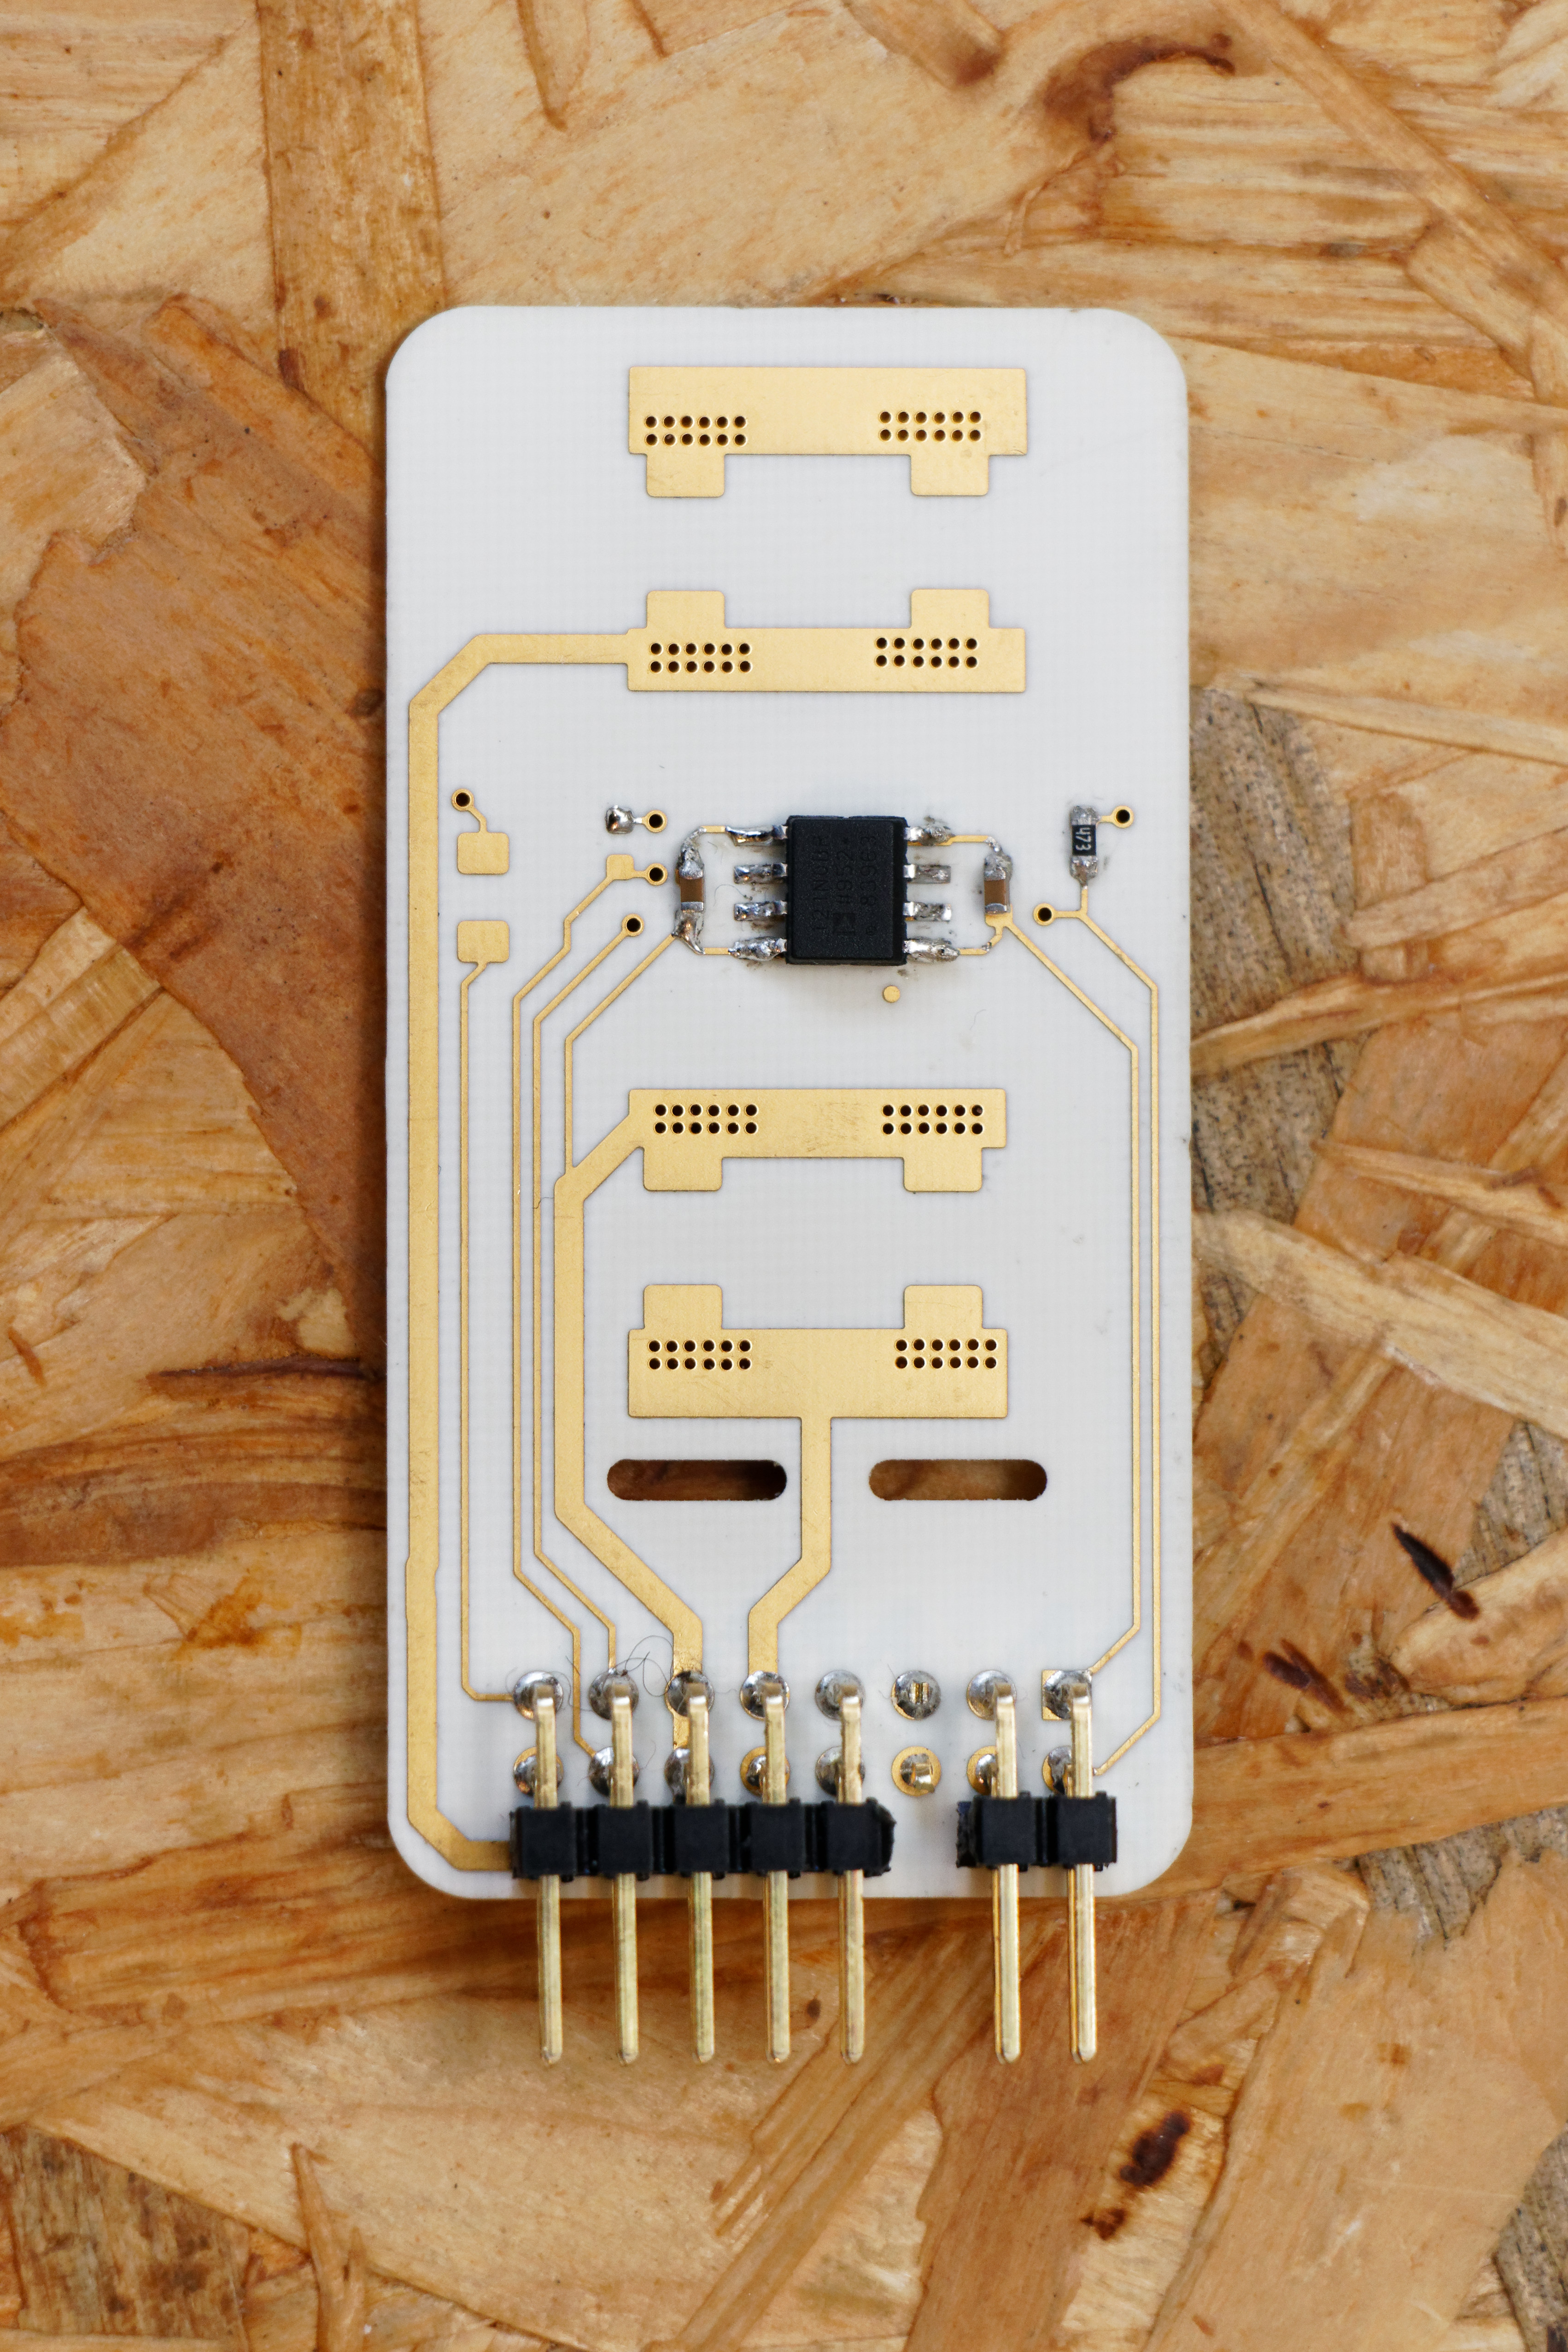
\includegraphics[max height=5cm,max width=0.95\linewidth]{imgDS/OTHER.jpg}% requires the graphicx package
%		\caption{ \chipID {} Functional schematic illustration. }
%		\label{fig.:SupplyVSDR}
%	\end{minipage}
%	\begin{minipage}[t]{0.5\linewidth}
%		\centering
%		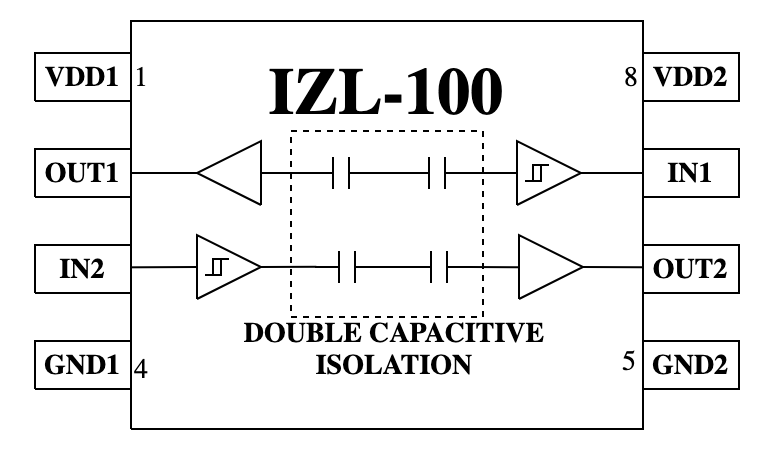
\includegraphics[max height=5cm,max width=0.95\linewidth]{imgDS/IZL100.jpg}% requires the graphicx package
%		\captionsetup{width=.9\linewidth}
%		\caption{Switching node illustration (yellow): DVDT = 100KV/ \textmu s}
%		\label{fig.:functional}
%	\end{minipage}
%\end{figure}


%\begin{figure}[!htb]
%	\begin{minipage}[t]{0.5\linewidth}
%		\centering
%		\captionsetup{width=0.9\linewidth}
%		\includegraphics[max height=5cm,max width=0.95\linewidth]{imgDS/009.png}% requires the graphicx package
%		\caption{ \chipID {} Functional schematic illustration. }
%		\label{fig.:SupplyVSDR}
%	\end{minipage}
%	\begin{minipage}[t]{0.5\linewidth}
%		\centering
%		\includegraphics[max height=5cm,max width=0.95\linewidth]{imgDS/010.png}% requires the graphicx package
%		\captionsetup{width=.9\linewidth}
%		\caption{Switching node illustration (yellow): DVDT = 100KV/ \textmu s}
%		\label{fig.:functional}
%	\end{minipage}
%\end{figure}
%
%Figure \ref{fig.:schematic} illustrates \chipID { } \blockID  schematic view.  
%\begin{figure}[!htb]
%	\centering
%	\includegraphics[max height=21cm,max width=18cm]{imgDS/009izl.png}
%	\caption{\chipID{ } - \blockID{ } -  Schematic view}
%	\label{fig.:schematic}
%\end{figure}
%
%Figure \ref{fig.:schematic} illustrates \chipID { } \blockID  schematic view.  
%\begin{figure}[!htb]
%	\centering
%	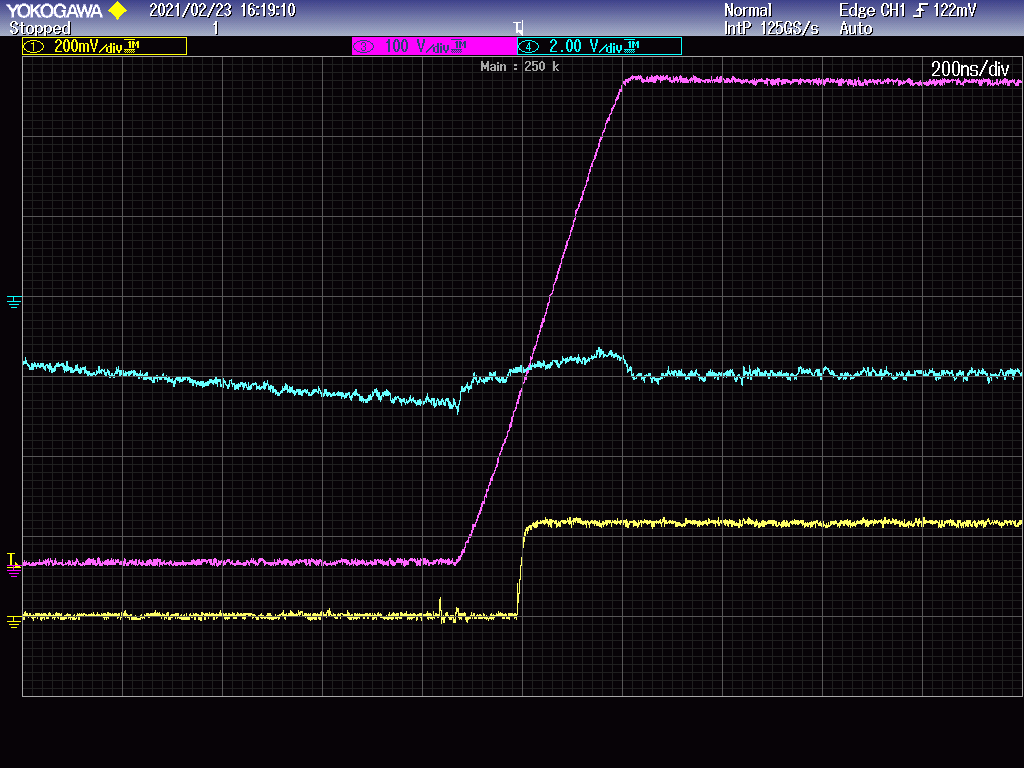
\includegraphics[max height=21cm,max width=18cm]{imgDS/010adum.png}
%	\caption{\chipID{ } - \blockID{ } -  Schematic view}
%	\label{fig.:schematic}
%\end{figure}
%
%\FloatBarrier
%\clearpage
%
%\pagebreak
%
%\section{Schematic }
%
%
%Figure \ref{fig.:schematic} illustrates \chipID { } \blockID  schematic view.  
%\begin{figure}[!htb]
%	\centering
%	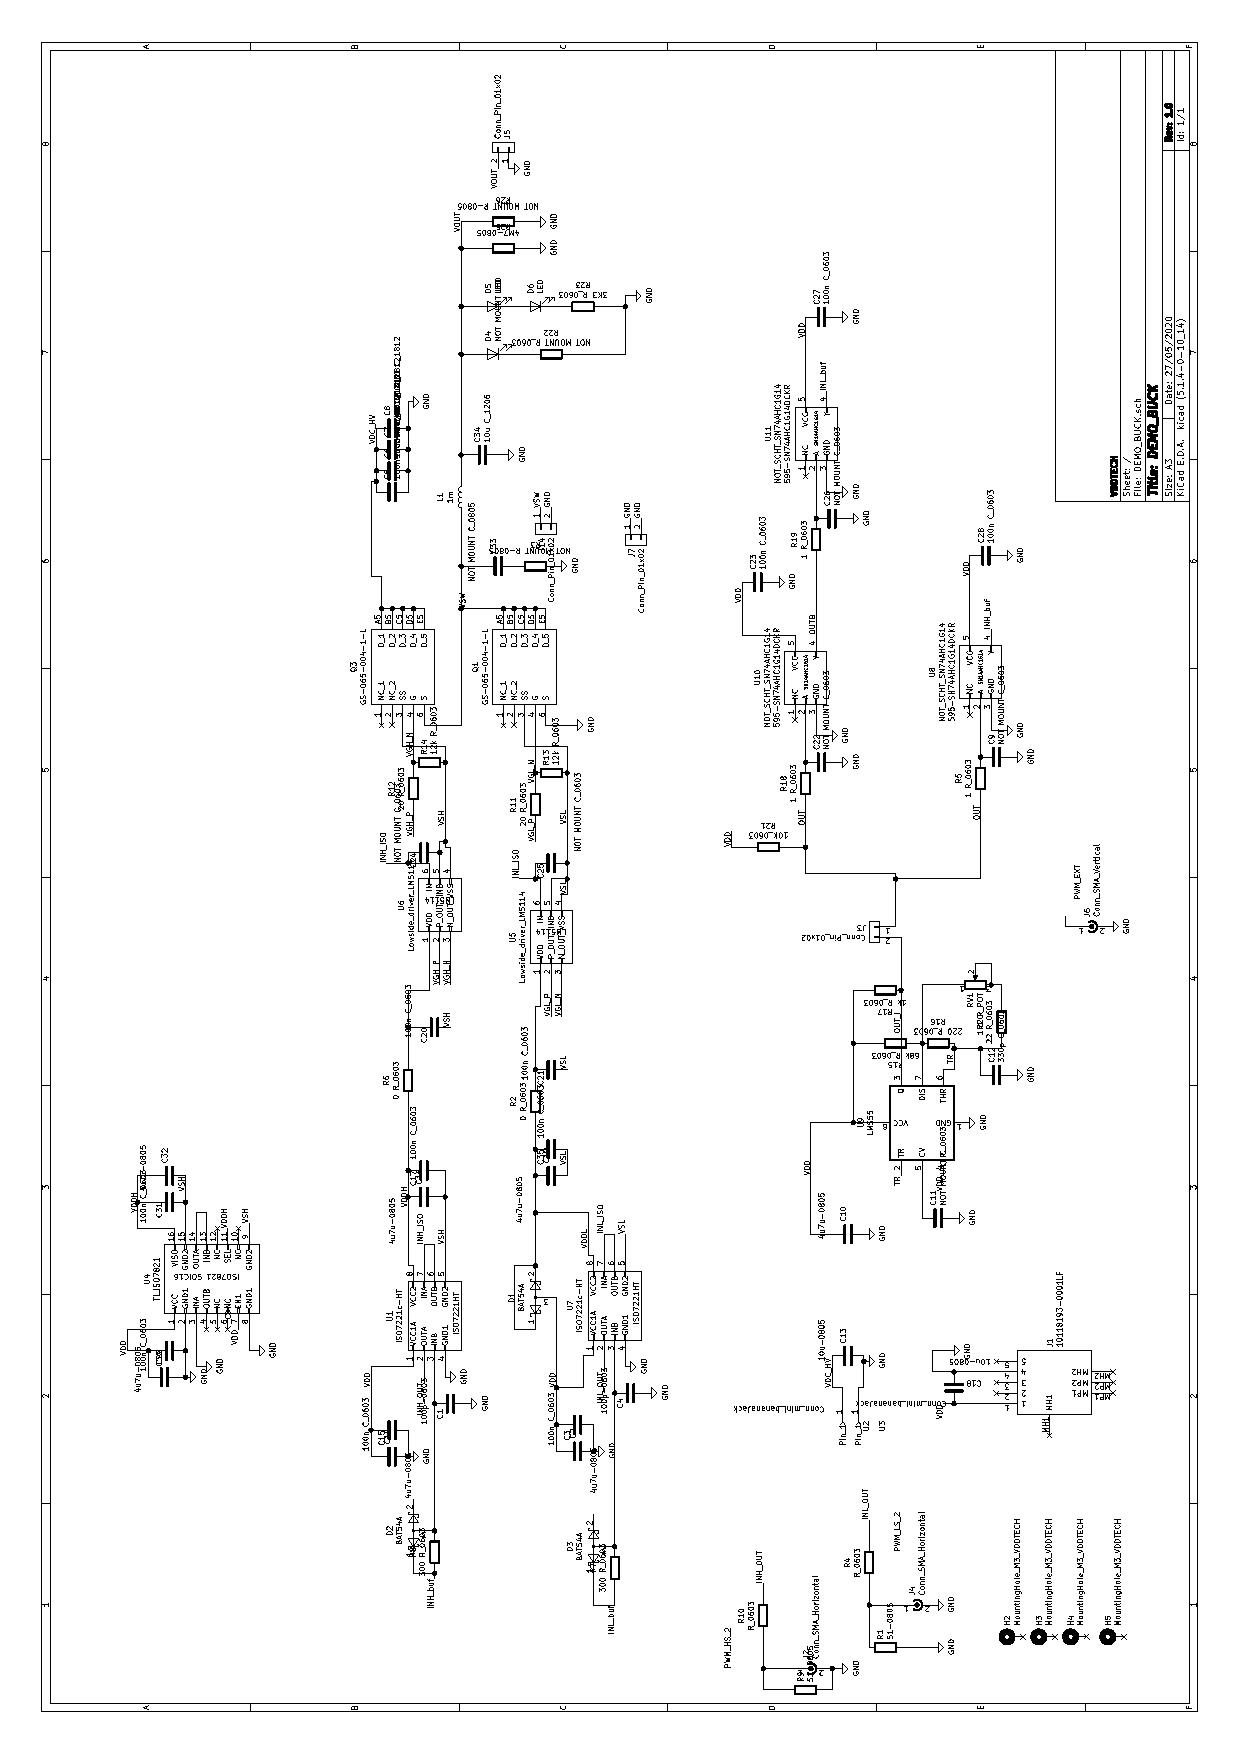
\includegraphics[max height=21cm,max width=18cm]{imgDS/schematic2.pdf}
%	\caption{\chipID{ } - \blockID{ } -  Schematic view}
%	\label{fig.:schematic}
%\end{figure}
%
%\FloatBarrier
%\clearpage
%
%\pagebreak 



%\section{Assembly drawing}
%Figure \ref{fig.:assembly} illustrates \chipID { } assembly view.  
%\begin{figure}[!htb]
%	\centering
%	\includegraphics[max height=21cm,max width=21cm,  angle =90]{imgDS/assembly.png} 
%	\caption{\chipID{ } - \blockID{ } -  assembly view}
%	\label{fig.:assembly}
%\end{figure}
%
%\pagebreak 
%
%\section{Bill of Materials }
%
%Figure \ref{fig.:BOM} summarizes \chipID { } main components references.  
%\begin{figure}[!htb]
%	\centering
%	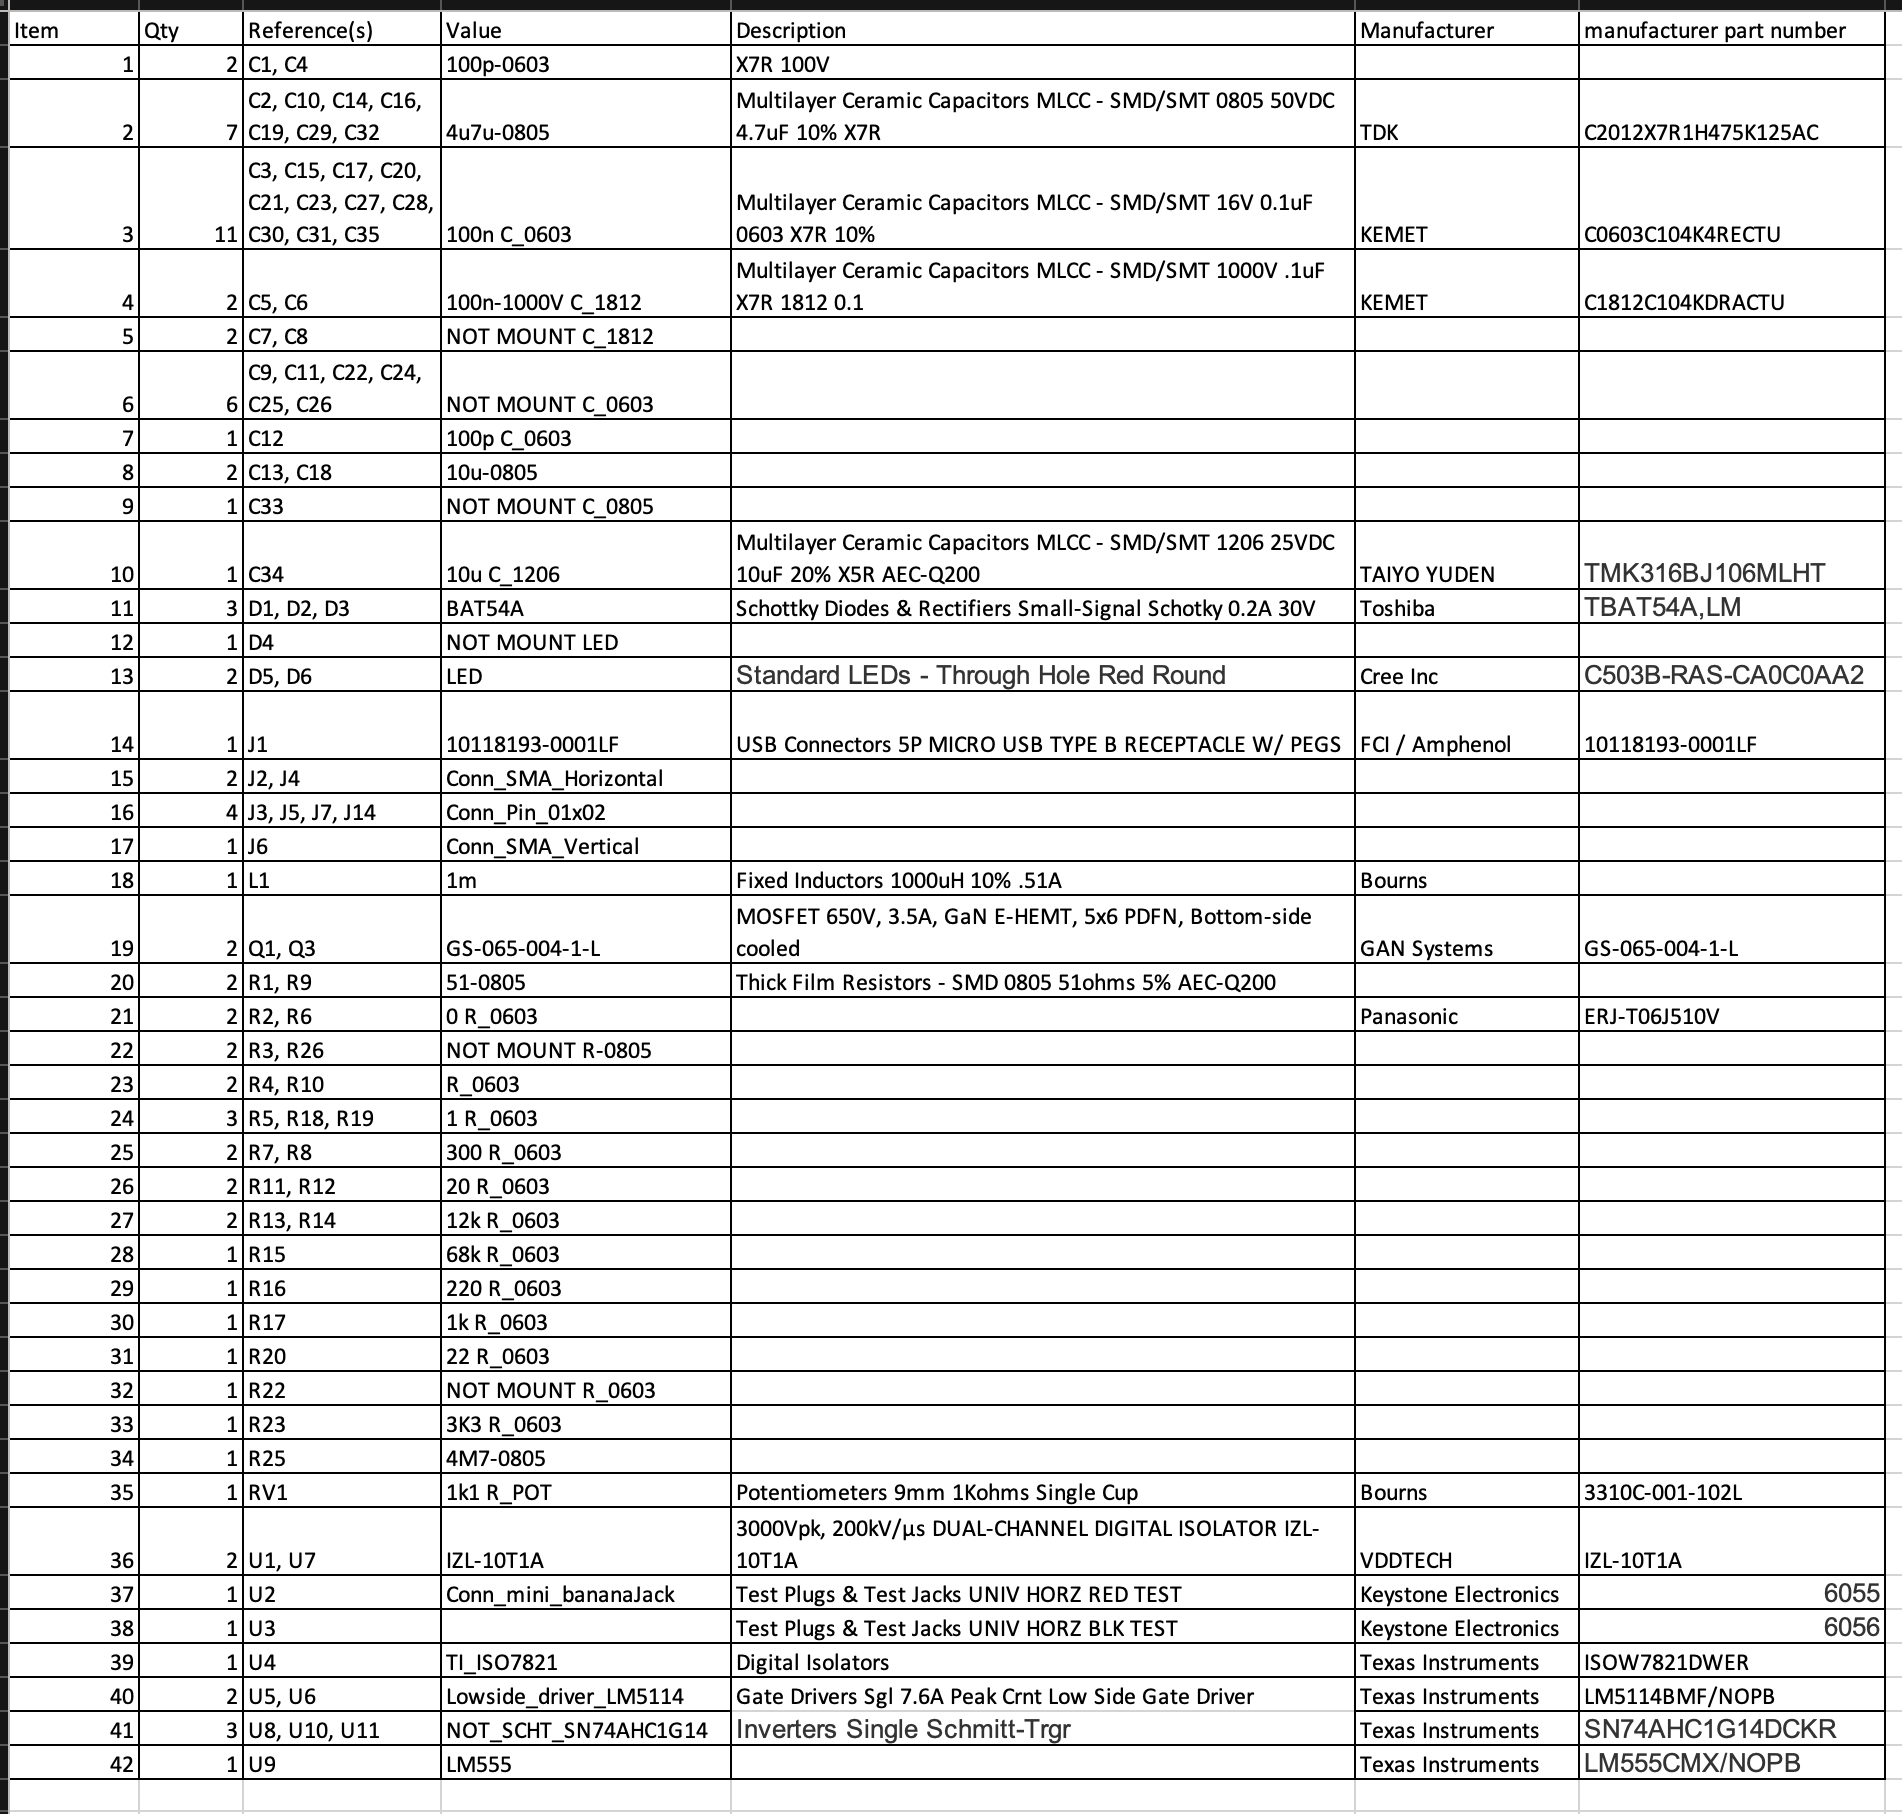
\includegraphics[max height=17cm,max width=18cm]{imgDS/BOM.png} 
%	\caption{\chipID{ } - Main components references }
%	\label{fig.:BOM}
%\end{figure}
%\pagebreak 

\end{document}
